\documentclass[b1]{sciposter}

\usepackage{graphicx}
\usepackage{multicol}

\usepackage[square,numbers]{natbib}


\title{Heavy Photon Search}
\author{S. Paul, M. Diamond}
\institute{College of William and Mary, SLAC National Accelerator Laboratory}
\conference{SLAC Summer Institute 2017}
\email{sebouh.paul@gmail.com, mdiamond@slac.stanford.edu}
%\author{R. Essig, C. Field, M. Graham, G. Haller, R. Herbst, J. Jaros, C. Kenney, T. Maruyama, K. Moffeit, T. Nelson, H. Neal, A. Odian, M. Oriunno, R. Partridge, S. Uemura, D. Walz}
%\institute{SLAC National Accelerator Laboratory, Menlo Park, CA 94025}
%\conference{Stanford Graduate Student Open House, April 5, 2011}
%\leftlogo{hps_logo}
%\leftlogo{slac_logo_vector}
%\rightlogo{JLab_logo_white}
\leftlogo{wm_logo_slac_logo_v}
\rightlogo{hps_logo_jlab_logo_v}

\newcommand{\YUGE}{\huge}

\renewcommand{\authorsize}{\YUGE}
\renewcommand{\instsize}{\large}

\begin{document}

\setlength{\logowidth}{0.15\textheight}
\setlength{\titlewidth}{\textwidth}
\addtolength{\titlewidth}{-2\logowidth}
\maketitle

%\large 
{The Heavy Photon Search (HPS) collaboration is performing an experiment aimed at discovering a hidden-sector heavy (or dark) photon - a $U(1)$ vector boson. Heavy photons (or $A'$s) couple to electric charge through kinetic mixing with the Standard Model photon, with production analogous to bremsstrahlung radiation. They may also mediate dark matter interactions. The HPS experiment has recently performed two successful engineering runs, first in spring of 2015 and later in the winter of 2016 with a higher beam energy. HPS is expected to take significantly more data during 2019. The experimental apparatus is composed of a six-layer silicon microstrip vertex tracker and a PbWO$_4$ crystal calorimeter. 
%HPS is a very small experiment by modern standards but uses cutting edge detection and readout technologies. HPS offers prospective HEP thesis students all aspects of experimental work, from design and hardware construction on numerous upgrade possiblities, to data taking and analysis.
}

\begin{multicols}{3}
	%\columnseprule=0mm
	\section*{Motivation}
Anomalies 
%from cosmic rays
%\cite{Finkbeiner:2010sm}, as well as 
in dark matter distributions in galactic haloes \cite{Vogelsberger:2012ku} provide motivation for a heavy photon in the 0.1 to 1.0 GeV range.  This particle is an example of a vector portal between Standard Model particles and the dark matter sector.  Depending on its parameters, it could be produced in a laboratory setting, and identified through its decay products.
% through electron-nucleus scattering via a process analogous to bremsstrahlung.  It could then decay into an lepton-antilepton pair, which may be identified through its narrow resonance, and possibly also the displacement of the decay.

\begin{figure}
\begin{center}
\makebox[\textwidth]{
\includegraphics[width=1.1\textwidth]{motivation_artsy_2.png}
%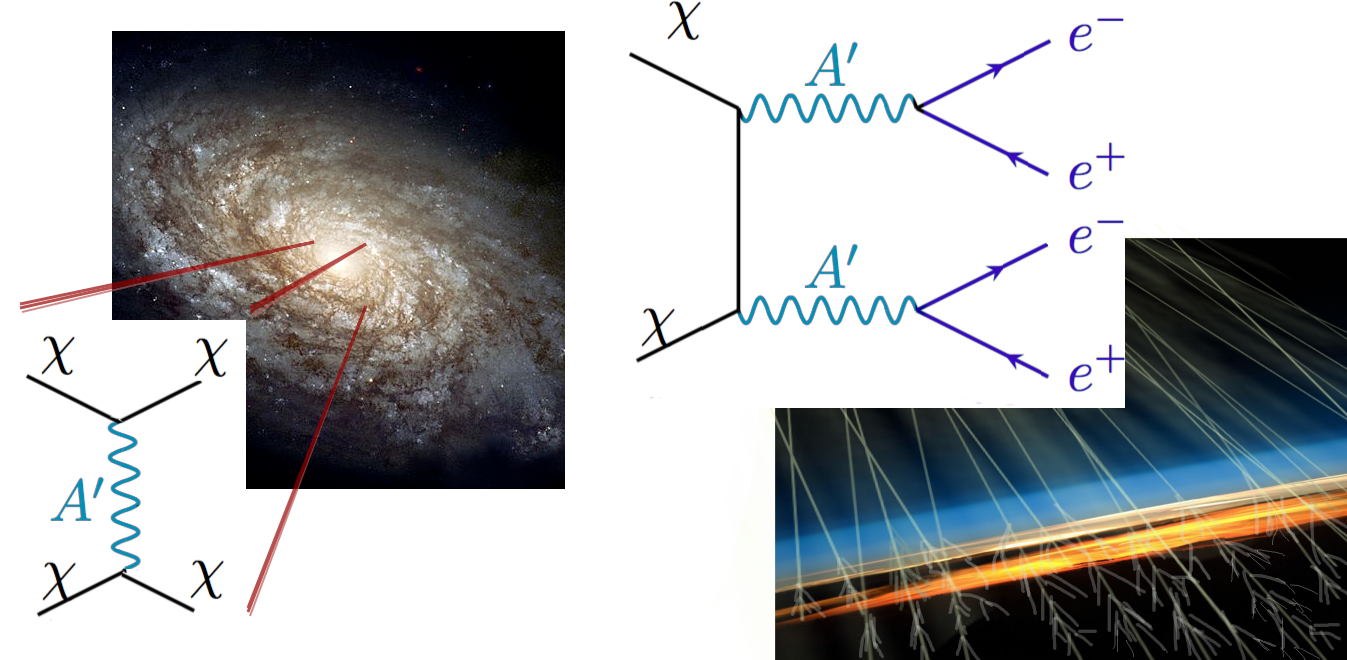
\includegraphics[width=.4\textwidth,trim={0cm, 0cm, 25cm, 0cm}, clip]{motivation_artsy_shower.png}%\hspace{1cm}
%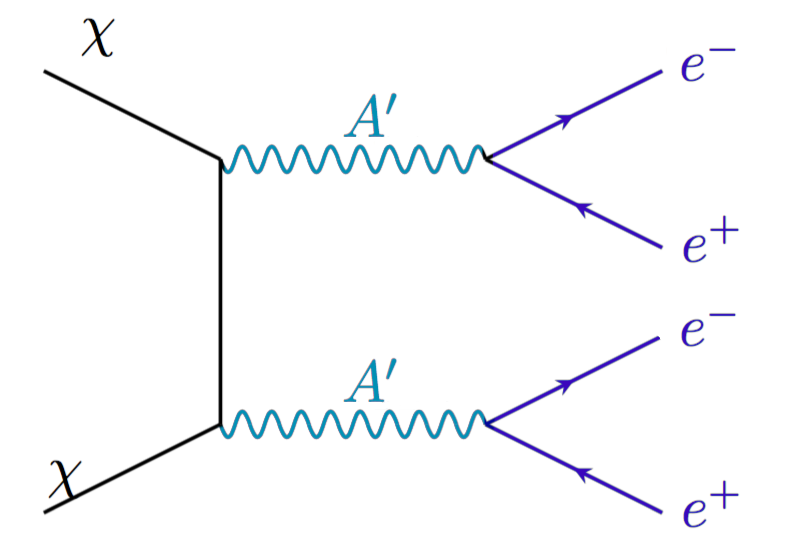
\includegraphics[width=0.63\textwidth]{dm_coannihilation}}
%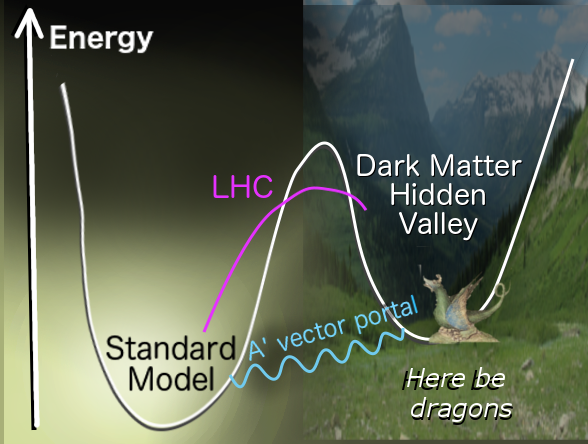
\includegraphics[width=.5\textwidth]{motivation_hidden_valley.png}
}
\label{default}
\end{center}
\caption{(left) Dark matter self-interaction, mediated by $A'$, which may solve ``core-cusp" anomalies in galactic haloes.  (right) %Dark matter annihilating into leptons through $A'$, as a solution to cosmic-ray anomalies.}
The heavy photon as a ``vector portal" between the Standard Model and a ``hidden vector" dark sector.}
\end{figure}

	%A heavy photon would be theoretically favorable in the mass range of 0.1 to 1.0 GeV, couple weakly to electrons, and decay to $e^+e^-$. It would be produced by electron bremsstrahlung on a heavy target, and be identified as a narrow $e^+e^-$ resonance. Weak couplings of this heavy photon to electrons account for it having not yet been discovered and can give rise to separated vertices in its decay, providing a secondary signature. Heavy photons have become a hot topic recently because they may provide an explanation to several recently observed astrophysical anomalies (e.g. gamma rays from the galactic center), and be intimately linked to dark matter annihilation.
        %explain high energy electrons and positrons in cosmic rays, and be intimately linked to dark matter annihilation.
	%We consider new sub-GeV mass vector bosons --- ``dark photons'' A' --- that couple very weakly to electrons (similar considerations apply to pseudo-vectors, scalars, and pseudo-scalars with sub-GeV mass that couple to electrons). It is useful to parameterize the coupling $g'$ of the A' to electrons by a dimensionless $\epsilon \equiv g'/e$, where $e$ is the electron charge. Cross-sections for A' production then scale as $\alpha'/\alpha = \epsilon^2$, where $\alpha'=g'^2/4\pi$ and $\alpha=e^2/4\pi$ are the fine-structure constants for the dark photon and ordinary electromagnetic interactions, respectively. This experiment will search for A' bosons with mass $m_{A'} \approx 100$ MeV and $\alpha'/\alpha \ge 10^{-5}$, which can be produced by a reaction analogous to photon bremsstrahlung and will decay promptly to $e^+e^-$ or other charged particle pairs.


	%\subsection*{Motivation for New Physics}
	%New light vector particles, matter states, and their associated interactions are ubiquitous in
	%extensions of the Standard Model. However, the symmetries of the Standard Model
	%restrict the interaction of ordinary matter with such new states. Indeed, most interactions
	%consistent with Standard Model gauge symmetries and Lorentz invariance have couplings
	%suppressed by a high mass scale. One of the few unsuppressed interactions is the coupling of
	%charged Standard Model particles $\psi$,
	%$$\Delta L = g'A'^\mu\bar{\psi}\gamma_\mu\psi$$
	%to a new gauge boson A', which is quite poorly constrained for small $g'$. Similar
	%couplings between the A' and other Standard Model fermions are also allowed, with relations
	%between their couplings (anomaly cancellation) required for the A' gauge symmetry to be
	%quantum-mechanically consistent. For example, the A' 
	%can have couplings proportional to the
	%electromagnetic charges $q_i$ of each fermion, $g_{qi} = \epsilon e_{qi}$.

	%Seeing such a new gauge boson would constitute the first discovery of a new gauge force since
	%the observation of Z-mediated neutral currents.

	%Besides the obvious physical interest of a fifth
	%force, the A' like the Z could open up a new ``sector'' of light, weakly coupled particles whose
	%spectrum and properties could be measured in fixed-target experiments and flavor factories.
	%The A' sector would provide a new laboratory for many physical questions, and would be
	%revealing precisely because its interactions with Standard Model particles are so weak. In
	%particular, if nature is approximately supersymmetric near the TeV scale, the mass scale of
	%supersymmetry breaking for the A' sector is naturally suppressed by $\epsilon$ times gauge couplings.
	%In this case, supersymmetry could be studied easily in the A' sector, and possibly even
	%discovered there by relatively low-energy experiments before Standard Model superpartners are
	%seen at colliders.

	%\subsection*{Dark Matter}
	%The WIMP dark matter hypothesis argues that if dark matter consists of
	%$\sim$100 GeV to 10 TeV particles interacting via the electroweak force (``weakly interacting massive
	%particles'' or ``WIMPs''), they would automatically have the right relic abundance observed
	%today. These observations are
	%also consistent with the hypothesis that dark matter interacts with ordinary matter through a
	%new force, mediated by a new 50 MeV --- 1 GeV mass gauge boson.

	%The satellites PAMELA and Fermi, the balloon-borne detector ATIC, the groundbased
	%Cerenkov telescope HESS, as well as other experiments, observe an unexplained excess in
	%the cosmic-ray flux of electrons and/or positrons.
	%Dark matter charged under a new gauge force and annihilating to A' pairs, which then decay to electron or muon pairs, explains these observations better than ordinary WIMP dark matter.

%	\subsection*{True Muonium}
%	This experiment has the potential to discover ``true muonium'' --- a bound state of a $\mu^+\mu^-$ pair. Positronium ($e^+e^-$) and muonium ($\mu^+e^-$) have been produced and studied, but true muonium, or dimuon, has not yet been detected.
	%True muonium is the most compact pure QED system whose decay is a pure QED process, since the muon lifetime (unlike the tau lifetime) is much longer than the QED decay time. True muonium is produced in either a singlet or a triplet state; it is the triplet state that is observable in this experiment.

	\section*{Signals and Backgrounds}
	\subsection*{Heavy Photon Signal}
%	\begin{figure}
%		\begin{center}
%			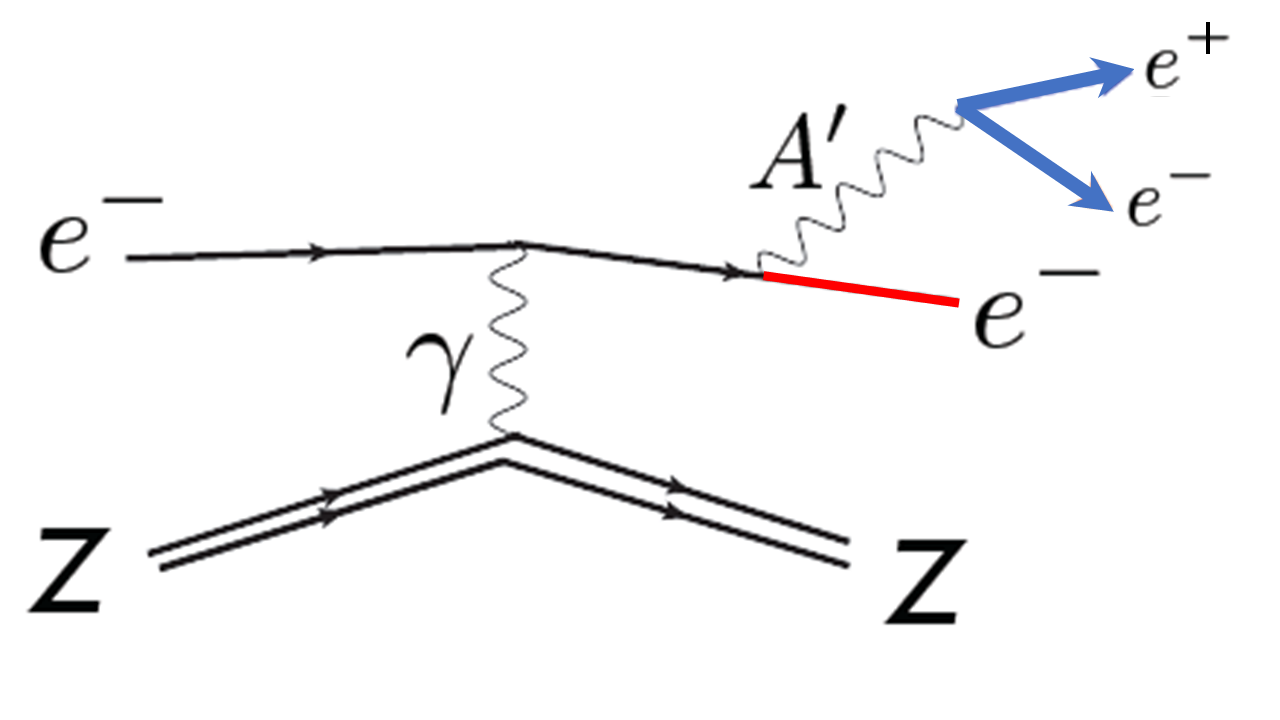
\includegraphics[width=0.5\textwidth]{signal}
%		\end{center}
%		\caption{A' production by bremsstrahlung off an incoming electron as it scatters on a nucleus with atomic number Z.}
%	\end{figure}
%
%	\begin{figure}
%		\begin{center}
%			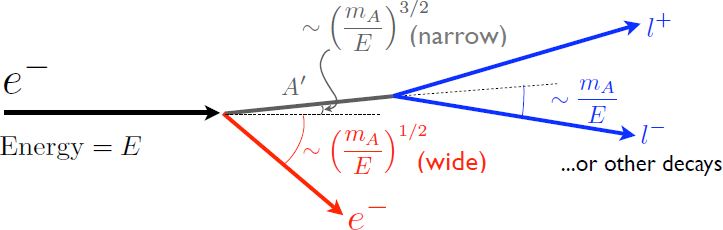
\includegraphics[width=\textwidth]{ap_kine}
%		\end{center}
%		\caption{A' production and decay kinematics.}
%	\end{figure}

\begin{figure}
		\begin{center}
			\makebox[\textwidth]{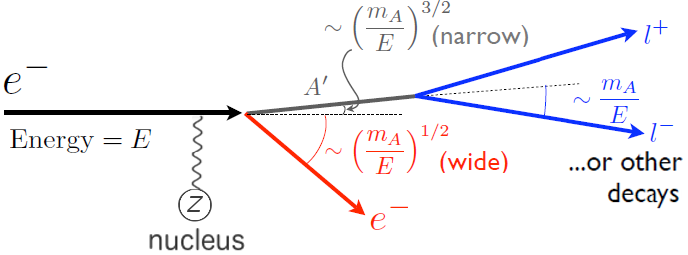
\includegraphics[width=1.1\textwidth]{ap_kine_topokinematics}}
		\end{center}
		\caption{Topology and kinematics of an $A'$ production as an incoming electron scatters off a nucleus with atomic number $Z$, and then decays.}
	\end{figure}


	$A'$ particles are generated in electron collisions on a fixed target by a process analogous to
	ordinary photon bremsstrahlung.
	%The major difference in the kinematics is that nearly the entire beam energy is carried by the produced A'.
	%The A' production rate is suppressed relative to photon bremsstrahlung by a factor of $\epsilon^2m_e^2/m_{A'}^2$.
	%A' emission is dominated at angles less than $\max(\sqrt{m_{A'}m_e}/E_0,(m_{A'}/E_0)^{3/2})$, and nearly the entire beam energy is carried by the produced A'.
	%A' particles decay to $e^+e^-$ or other charged particle pairs. The decay length varies from prompt to tens of cm, depending on $\epsilon$ and $m_{A'}$. The opening angle of the decay products is on the order of $m_{A'}/E_0$.


	%\subsection*{True Muonium Signal}
	%The triplet states of true muonium decay to $e^+e^-$ with a rest frame lifetime of 1.81$n^3$ ps. With a beam energy of 6.6 GeV, the typical decay length of the $n=1$ state would be 1.7 cm. The kinematics of the true muonium signal is similar to that of A'. 

	%For the nominal running conditions of $E_{beam}=5.5$ GeV, 400 nA beam current, $3\times10^6$ s running time and a single target foil, we can expect to produce 20 $n=1$ triplet true muonium states, of which we would expect to see 2 (accounting for all efficiencies) with vertices sufficiently separated from the target. Using multiple target foils and a higher beam current would scale this number linearly.

	%The triplet production cross-section scales with $Z^2$. The dissociation cross-section of true muonium is very large and also scales like $Z^2$. This means that the production rate is independent of $Z$ and also of the target thickness (since only the true muonium produced in the last fraction of a thick target will escape before breaking apart).

	\subsection*{Backgrounds}
	\begin{figure}
		\begin{center}
			\makebox[\textwidth]{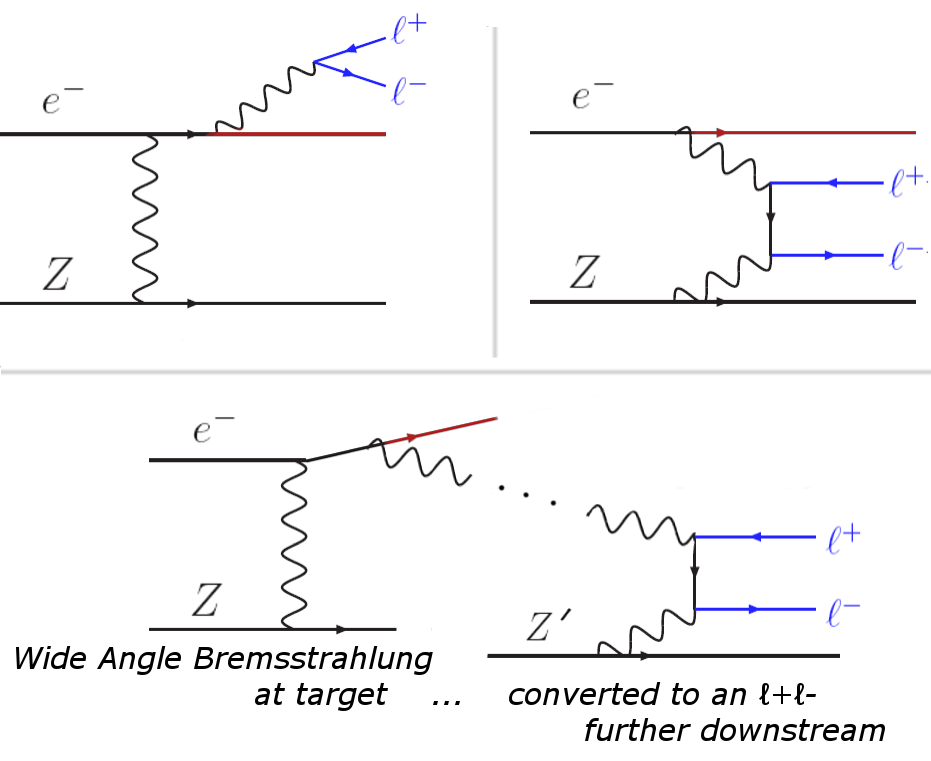
\includegraphics[width=1.1\textwidth]{trident_wab}}
		\end{center}
		%\caption{Sample diagrams of (top left) radiative trident ($\gamma^*$), (top right) Bethe-Heitler trident, and (bottom) converted wide-angle bremsstrahlung reactions, that comprise the primary QED background to $A'\to l^+l^-$ search channels.}
		\caption{Sample diagrams of QED background events: (top-left) radiative trident ($\gamma^*$), (top-right) Bethe-Heitler trident, and (bottom) converted wide-angle bremsstrahlung reactions}
	\end{figure}

%	QED tridents produce $e^+e^-$ pairs with nonzero invariant mass.  Additionally, photons produced via wide-angle bremsstrahlung are often converted to $e^+e^-$ pairs either in the target or in one of the layers of the silicon tracker.  These events are the dominant background to the A' signal, while a smaller component of our background is beam background due to our high beam current.  

%There are three main sources of background in our detector.  The first source are QED tridents, which produce $e^+e^-$ pairs at the target.  Secondly, photons produced via wide-angle bremsstrahlung are often converted to $e^+e^-$ pairs either in the target or in one of the layers of the silicon tracker.  Thirdly, beam background is non-negligible due to our high beam current.
	%Radiative tridents have identical kinematics to A' events. The A' events can only be separated by their invariant mass (resonance search) or by their decay length (displaced vertex search).
	%The Bethe-Heitler process has a much higher total cross-section than either A' production or radiative tridents, but the associated background can be significantly reduced because of its different kinematics.

	%\columnbreak
%	\subsection*{Beam Backgrounds}
%	\begin{figure}
%		\begin{center}
%			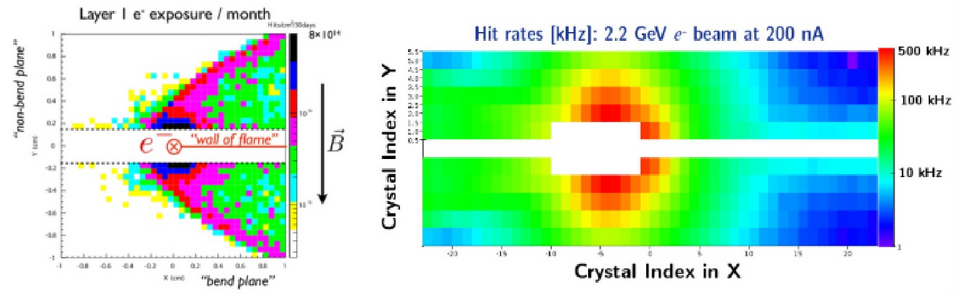
\includegraphics[width=1.0\textwidth]{background_hits}
%			%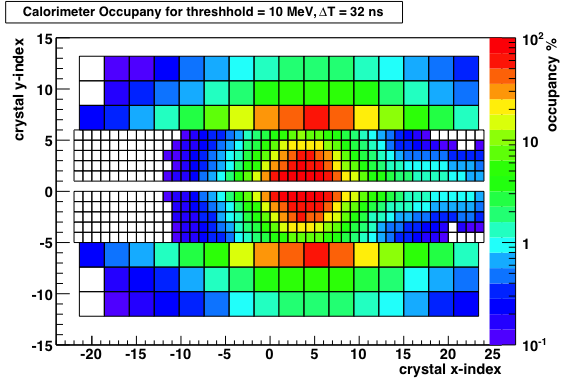
\includegraphics[width=0.55\textwidth]{ecal_background}
%		\end{center}
%		\caption{Beam background rates in Layer 1 on the silicon tracker (left) and the electromagnetic calorimeter (right).}
%	\end{figure}
%
%	Beam backgrounds are significant because of our high beam current and forward detector coverage.
	%Multiple Coulomb scattering and bremsstrahlung generate high fluxes of electrons and photons in the very forward direction,
	%and M{\o}ller scattering of atomic electrons generates high intensity low-energy electrons.
	%Electrons scattered in the target are bent by the dipole magnetic field to form a ``sheet of flame'' in the bend plane, creating a dead zone of $\pm$ 15 milliradians in which no detectors can be placed.

        \columnbreak
	\section*{Experimental Setup}
	\begin{figure}
		\begin{center}
			%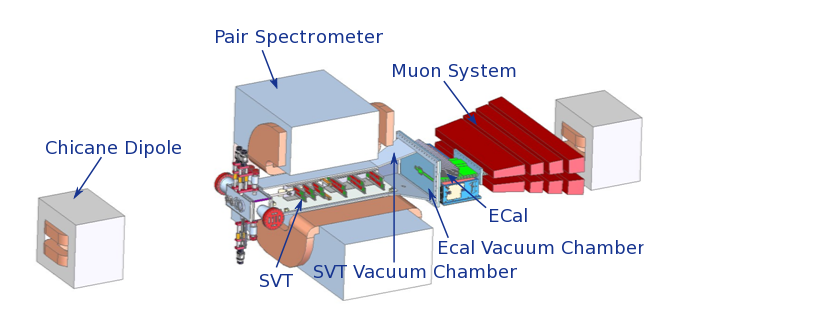
\includegraphics[width=1.2\textwidth]{HPS_detector_prop2014}
                        \makebox[\textwidth]{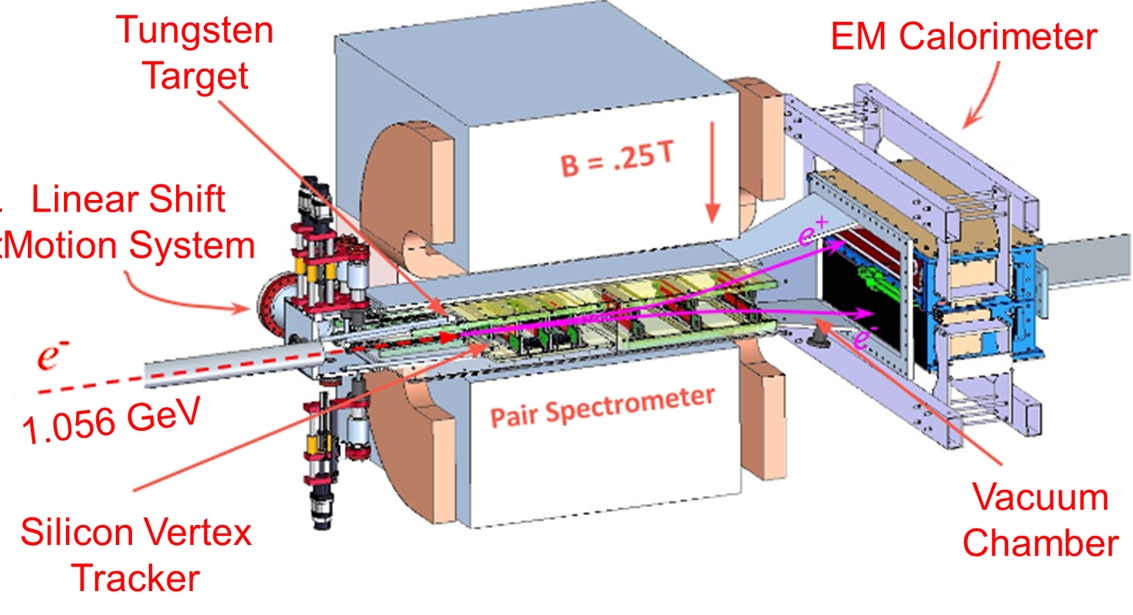
\includegraphics[width=1.1\textwidth]{hps_detector}}
			\caption{Schematic view of the HPS detector.}
		\end{center}
	\end{figure}

	%High luminosities and thin targets are needed to minimize beam background while maximizing A' production.
	The near-continuous duty cycle of the CEBAF beam at Jefferson Lab, along with fast detectors and electronics, allows us to run with short time windows and reduce occupancies.

	%Sensitivity to dark photons relies upon the precision measurement of two quantities in this
	%experiment: the invariant mass of the A' decay products and the position of the decay vertex. By
	%placing a tracking and vertexing detector immediately downstream of the target inside an
	%analyzing magnet, one obtains the complete kinematic information required for A'
	%reconstruction from a single system.

	%A fast and selective trigger is needed to reduce the sheer amount of data produced by the detectors. An electromagnetic calorimeter will select high-energy $e^+e^-$ events,
	%while a muon detection system will select $\mu^+\mu^-$ events.



	%\subsection*{Beamline and Target}
	%The HPS setup will be located behind the CLAS detector, in the downstream alcove of Hall B. The setup will be based on a three-magnet chicane, the second dipole magnet (pole length 91.44 cm, max field 1.15 T) serving as the analyzing magnet. The target foil will be positioned at the beginning of the high-field region of the analyzing magnet, and the silicon vertex tracker will be inside the magnetic field.

	%Production data taking will use a five-pass electron beam, at $\sim$5.5 GeV and with currents from 100 nA to 700 nA, incident on tungsten targets of thickness from 5 $\mu m$ (0.14\% RL) to 35 $\mu m$ (1\% RL).
	%The proposed luminosity for production running is $1.4 \times 10^{32}$ cm$^{-2}$ s$^{-1}$ per nucleus.



	\subsection*{Silicon Vertex Tracker}
	\begin{figure}
		\begin{center}
			\makebox[\textwidth]{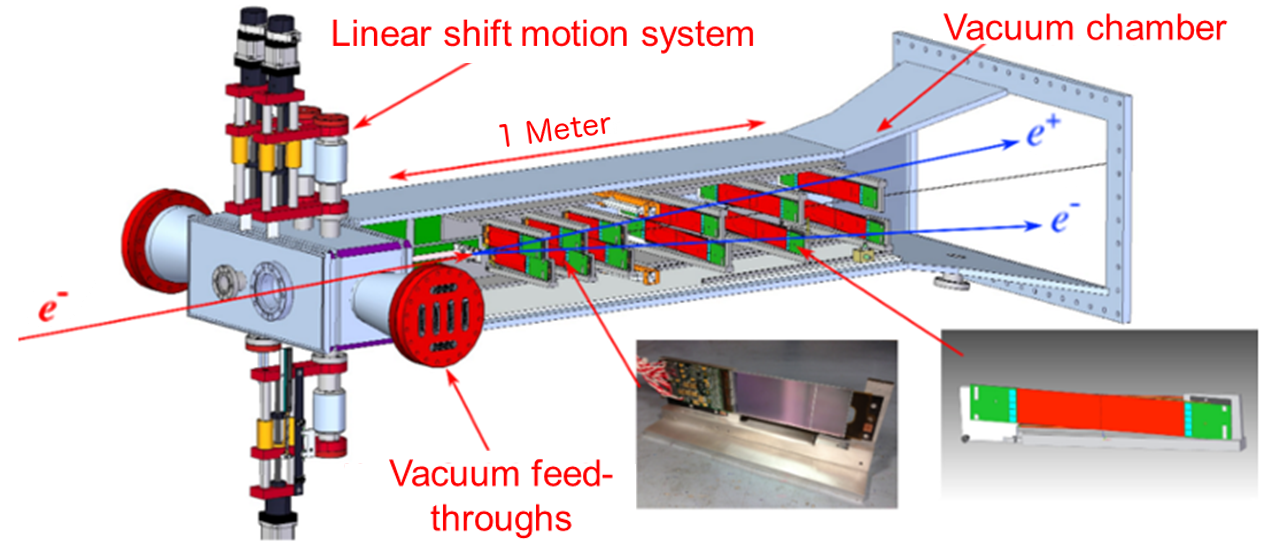
\includegraphics[width=1.1\textwidth]{svt_2014_labelled}}
			%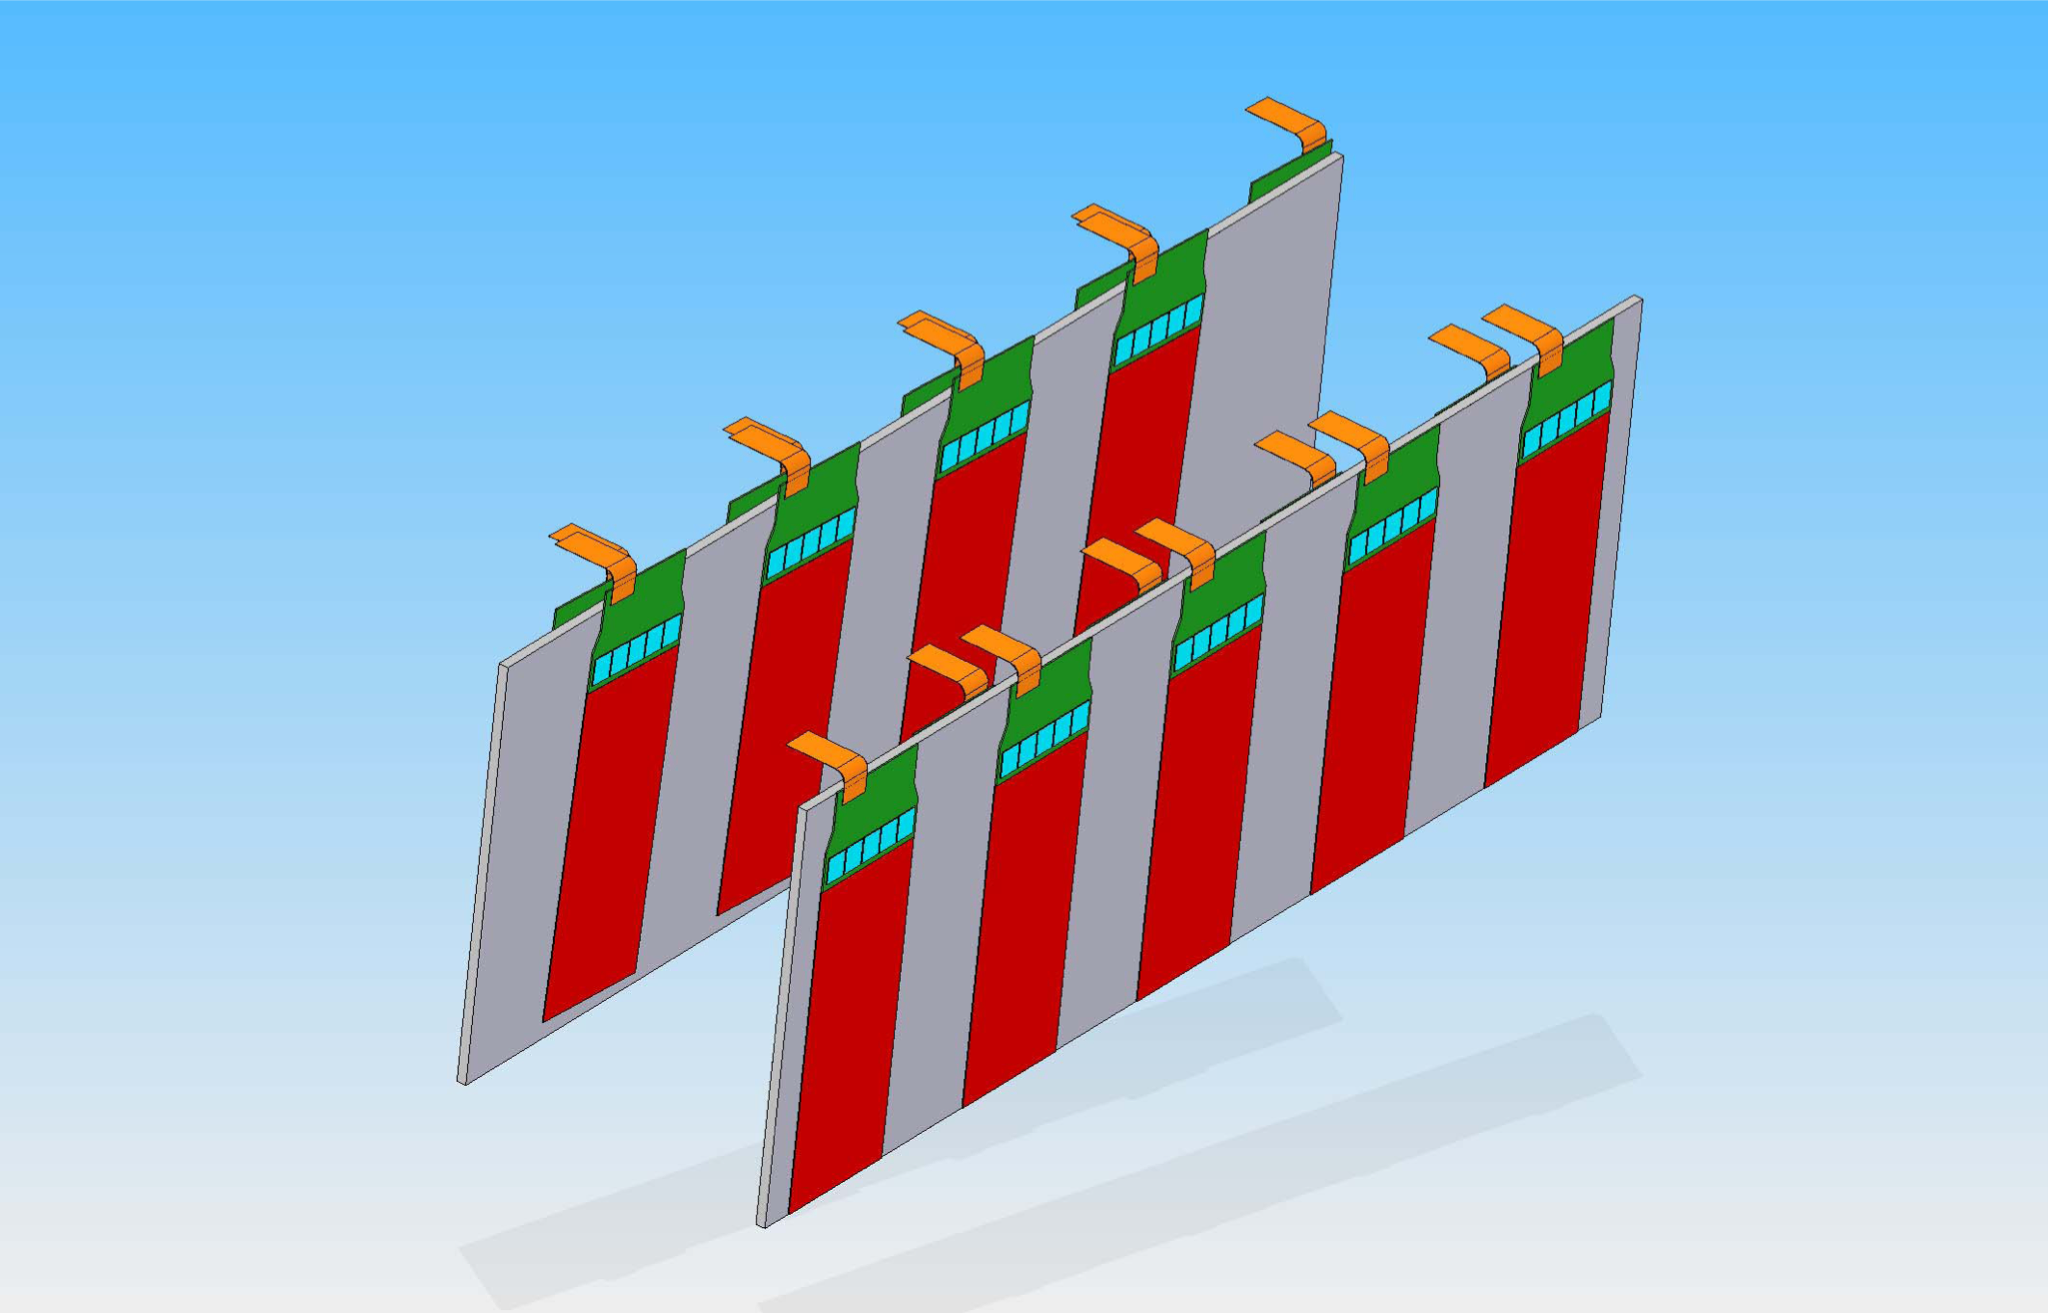
\includegraphics[width=0.45\textwidth]{si_module}
		\end{center}
		\caption{Renderings of the target assembly and silicon planes inside their support box.}
	\end{figure}

	%The thickness of material in the tracker are minimized to reduce measurement uncertainties and backgrounds.
	%The best choice is silicon microstrip sensors, which are simple, low-mass and fast.
	%We use 4 cm $\times$ 10 cm silicon sensors left over from the cancelled Run IIb upgrades at the Tevatron, and
	%the APV25 readout chip developed for the CMS tracker at the LHC, which can read out continuously at 40 MHz.

	%We will use 4 cm $\times$ 10 cm silicon sensors left over from the cancelled Run IIb upgrades at the Tevatron. These are radiation-tolerant and have a fine readout pitch, suitable for our high density of hits.

	%For readout, we will use the APV25 chip developed for the CMS tracker at the LHC, which can read out continuously at 40 MHz.
	%High signal-to-noise ratio (approximately 34 before irradiation) will extend the useful life of the sensors as radiation damage degrades performance.
	%We will use the chip's ``multi-peak'' readout mode, where the shaper output is sampled six times (once per clock cycle) after a trigger is received.
	%This allows us to fit the known shaper output curve to the samples, measuring peak amplitude and hit t0, and deconvoluting overlapping hits.
	%For each silicon sensor, five APV25 chips will be mounted on a hybrid circuit board. The design of this hybrid will be based on the hybrids used for the CMS Tracker Inner Barrel.

	%     The tracker is made up of six measurement layers. %at distances of 10, 20, 30, 50, 70, and 90 cm downstream from the target.
	%Each layer has two closely spaced planes of silicon microstrip sensors; one measures the bend plane coordinate
	%for momentum measurement, and the other (at an angle to the first) provides stereo resolution for track identification.
	Each of the SVT's six measurement layers has two closely-spaced planes of silicon microstrip sensors to measure both $X$ and $Y$ coordinates for momentum measurement and track identification. \cite{Adrian:2015hst}
	% Linear shift motion system allows SVT layers 1-3 to be moved within 15 mrad of the beam.
	%Each plane is divided into a top and a bottom module to accomodate the dead zone. A module comprises a composite support structure, silicon sensors, hybrid boards, and water-glycol cooling.
	%The hybrids and cooling tubes are located at the outside edges of the modules to keep them outside the high-flux region of the tracker.
	%The top and bottom halves of each layer are mounted to piezo motors so the vertical gap can be controlled.



	\subsection*{Electromagnetic Calorimeter}
	\begin{figure}
		\begin{center}
			%\includegraphics[width=0.8\textwidth]{ECal_looking_downstream}
			\makebox[\textwidth]{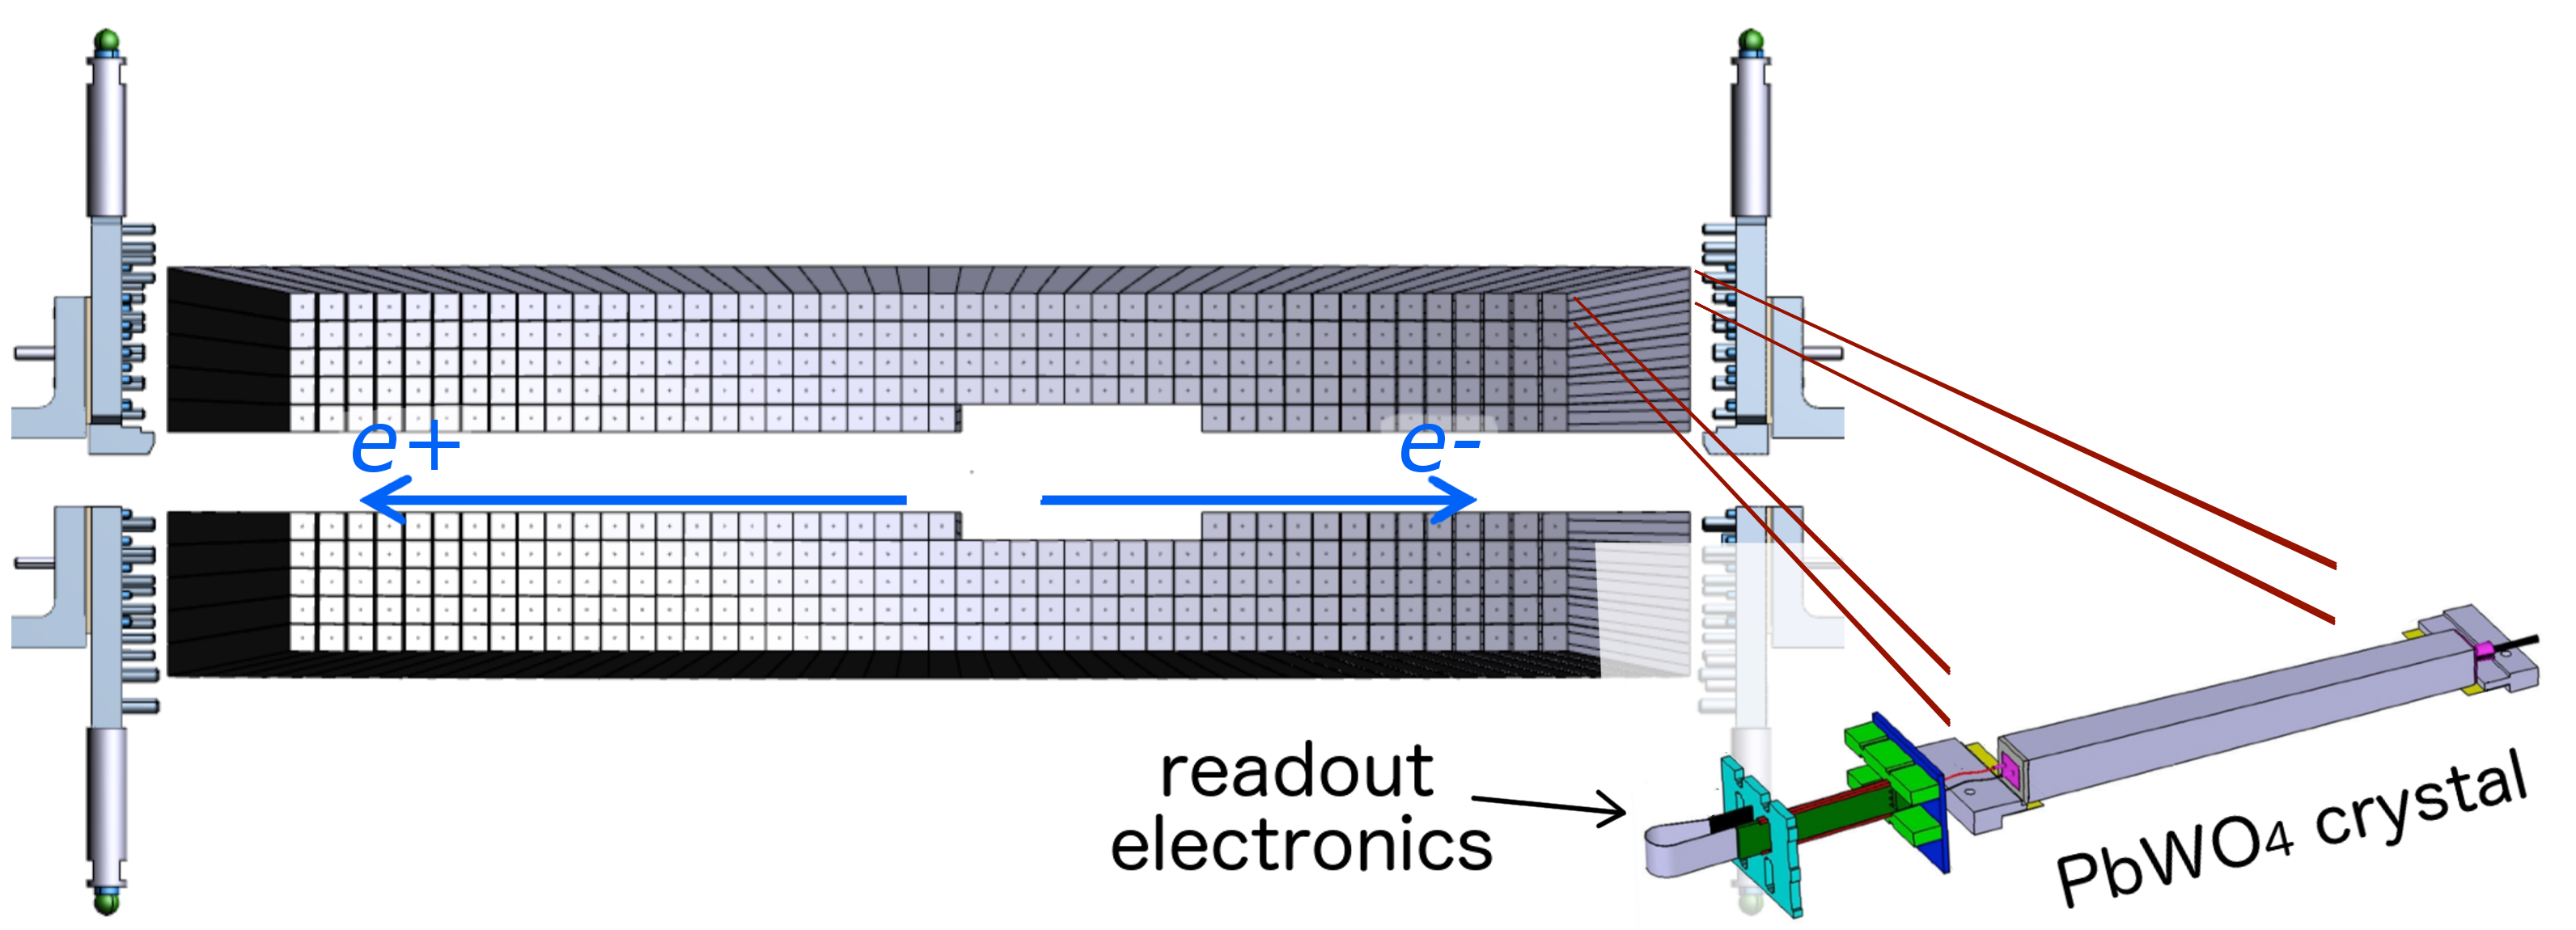
\includegraphics[width=1.1\textwidth]{Ecal_annotated}}
                        %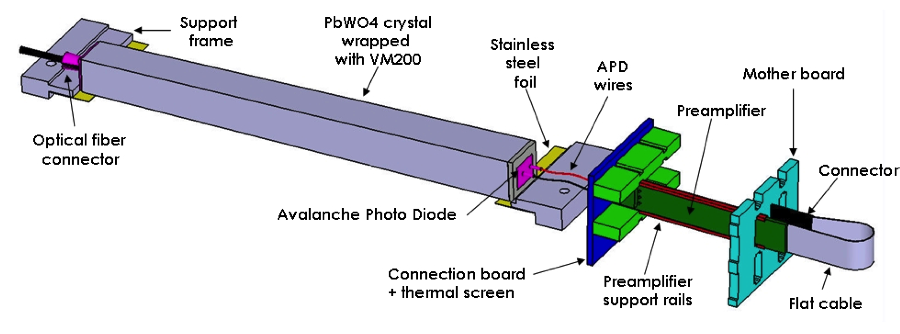
\includegraphics[width=0.47\textwidth]{ecal_module}
		\end{center}
		\caption{A rendering of the electromagnetic calorimeter (Ecal) setup looking down the beam line. %(left) and a more detailed view of the Ecal crystal. 
		
		% The front exit window and side plates are rendered transparent to permit a view of the crystals and the vacuum plates.
		}
	\end{figure}
	
The Ecal covers almost the full acceptance region of the SVT and is used for the data acquisition trigger, and also electron identification during the data analysis. \cite{Balossino:2016nly}
	
	%ECal will be positioned after the
	%analyzing dipole magnet, with the front face $\sim$130 cm downstream of the target, and will cover the full acceptance region of the silicon tracker.

	%Since the
	%area near the beam plane is under the highest radiation load, the modules near it must be
	%radiation resistant and should have finer granularity. 

	%\begin{figure}
	%	\begin{center}
	%		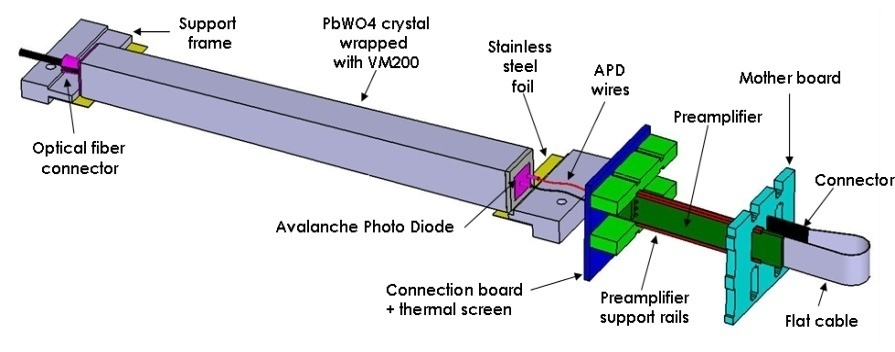
\includegraphics[width=0.45\textwidth]{pbwo4}
	%		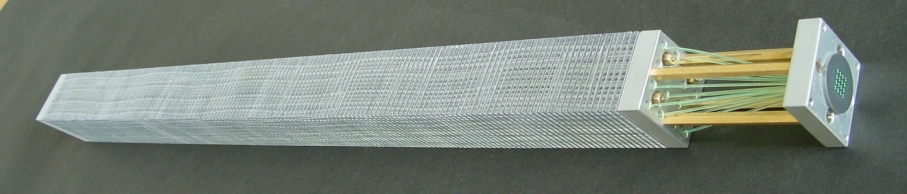
\includegraphics[width=0.45\textwidth]{shashlyk}
	%	\end{center}
	%	\caption{Lead tungstate (left) and shashlyk (right) detectors for use in the electromagnetic calorimeter.}
	%\end{figure}

	%We use lead tungstate (PbWO$_4$) crystals read by Hamamatsu avalanche photodiodes. %conventional PMT photodetectors in the outer region.

	%The lead tungstate (PbWO$_4$) crystals read by avalanche photodiodes that we are
	%planning to use are from the CLAS inner calorimeter (IC) and they fully meet the latter
	%requirements. The outer three rows in each half will be covered by larger, lead-glass or
	%``shashlyk'' type modules read by conventional PMT photodetectors.

	%\subsection*{Muon System}
	%Searching for the A' in its di-muon decay mode has the advantage of having greatly reduced
	%electromagnetic backgrounds for triggering. As a possible upgrade, the muon detection system will be installed behind
	%the ECal
	%and consists of four iron
	%absorbers and four scintillator planes positioned after each absorber layer.
	%Each scintillator plane will be made up of extruded
	%scintillator strips with embedded wave-shifting fiber readout.
	%The light will be detected from both ends of the strip using multi-anode photomultipliers. Signals from each channel will be sent to a TDC and to a
	%FADC. The FADC information will be used to construct the muon trigger. The TDC information
	%will be used in offline analysis to measure the hit position along the strip.

	%The ECal absorbs most of the electromagnetic background produced in the target. The
	%remainder will be attenuated by the first absorber layer of the muon system. Remaining
	%backgrounds will arise from photoproduction of $\pi^+$ and $\pi^-$ pairs in the target.
	%Most pions will shower
	%in the IC and in the iron absorbers and will not reach all way to the last layers of the scintillation
	%hodocopes, while most muons will pass through most or all of the layers of the system.

%	\subsection*{Electronics and DAQ}
%	%\begin{figure}
%	%	\begin{center}
%	%		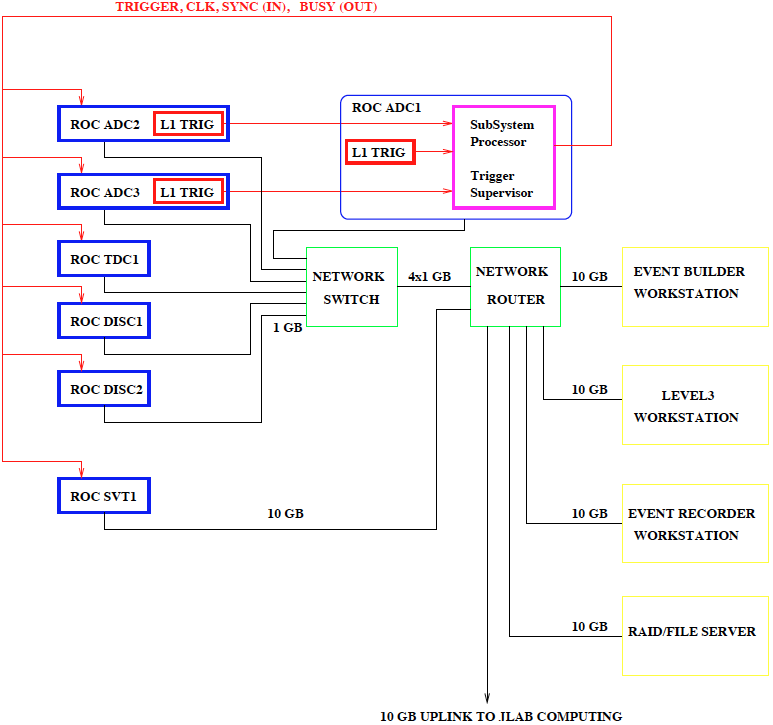
\includegraphics[width=0.8\textwidth]{daq}
%	%	\end{center}
%	%	\caption{Readout and processing system block diagram.}
%	%\end{figure}
%
%	A level 1 hardware trigger selects events to be read out. The triggered events are acquired and processed in the data acquisition and processing system. The DAQ system is designed for a maximum trigger rate of 50 kHz; simulations estimate that the ECal trigger rate due to background will be approximately 17 kHz.
	%There are three front-end electronics systems: an Electromagnetic Calorimeter (ECal) system, a Silicon Vertex Tracker (SVT) system, and a Muon system. A level 1 hardware trigger selects events to be read out. Only the ECal and the Muon system provide inputs to the Level 1 trigger system. The triggered events from the three subsystems are acquired and processed in the data acquisition and processing system. The events are down-selected in a Level 3 filter processing farm and the remaining events are transferred to the offline storage. The DAQ system is designed for a maximum trigger rate of 50 kHz; simulations estimate that the ECal trigger rate due to background will be approximately 17 kHz.

	%\begin{figure}
	%	\begin{center}
	%		\begin{tabular}{|c|c|c|c|}
	%			\hline
	%			Trigger cut & A' acceptance & Bkgd acceptance & Bkgd rate \\
	%			\hline
	%			At least two opposite clusters & 44.6\% & 1.26\% & 1.6 MHz\\
	%			Energy > 500MeV and < 4400 MeV & 46.4\% & 1.26\% & 0.3 MHz\\
	%			Energy sum < 5100 MeV & 46.4\% & 0.239\% & 120 kHz\\
	%			Energy difference < 3200 MeV & 46.1\% & 0.0959\% & 102 kHz\\
	%			Lower energy-distance slope cut & 45.4\% & 0.0823\% & 75 kHz\\
	%			Clusters coplanar to 45$^\circ$ & 44.6\% & 0.0601\% & 43 kHz\\
	%			Drop crystals in row 1, column 0,3,4 & 41.3\% & 0.0344\% & 20 kHz\\
	%			Not counting double triggers & 38.1\% & 0.0158\% & 17 kHz\\
	%			\hline
	%		\end{tabular}
	%	\end{center}
	%	\caption{Trigger selection cuts and their effect on the A' acceptance and background rate, as a percentage of the total number of simulated events. An A' mass of 250 MeV was used for this illustration.}
	%\end{figure}
\begin{small}
\bibliography{Biblio}
	
\bibliographystyle{apsrev}              % Indicate the sort by citation order style
%\bibliographystyle{plain} 
\end{small}
\columnbreak
	\section*{Experimental Reach}
Our experiment searches for $A'\to e^+e^-$, with or without a displaced vertex, depending on the coupling $\alpha'$:
\begin{small}
\begin{itemize}

	%In a resonance search, exclusion power is determined by the ratio of the signal within an invariant mass window to $\sqrt{N_{bin}}$, where $N_{bin}$ is the total background statistics in the same window. 
\item A resonance search is sensitive at large values of $\alpha'$, where the A' production rate is high.
\item A displaced-vertex search is sensitive at lower $\alpha'$, where decay lengths are longer than the the tails of the vertex distribution of prompt tridents.
\end{itemize}
\end{small}
	
	%	The sensitivity of a vertexing search is dependent on whether a signal event is detected with $z>zcut(m_{A'})$, where $zcut(m_{A'})$ is a mass-dependent value such that the expected background in each resolution-limited mass window $\delta m_{A'}$, with reconstructed vertices beyond this cut, does not exceed 0.5 events in the $3\times10^6$ s run period.
	\begin{figure}
		\begin{center}
			%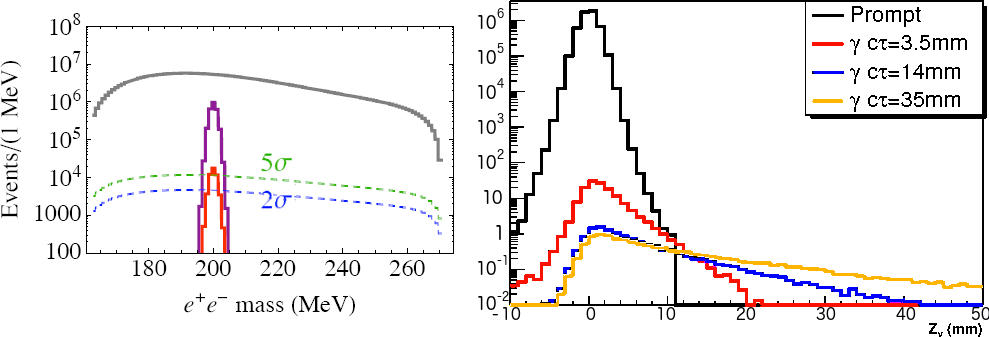
\includegraphics[width=1.05\textwidth]{s_b}
\makebox[\textwidth]{	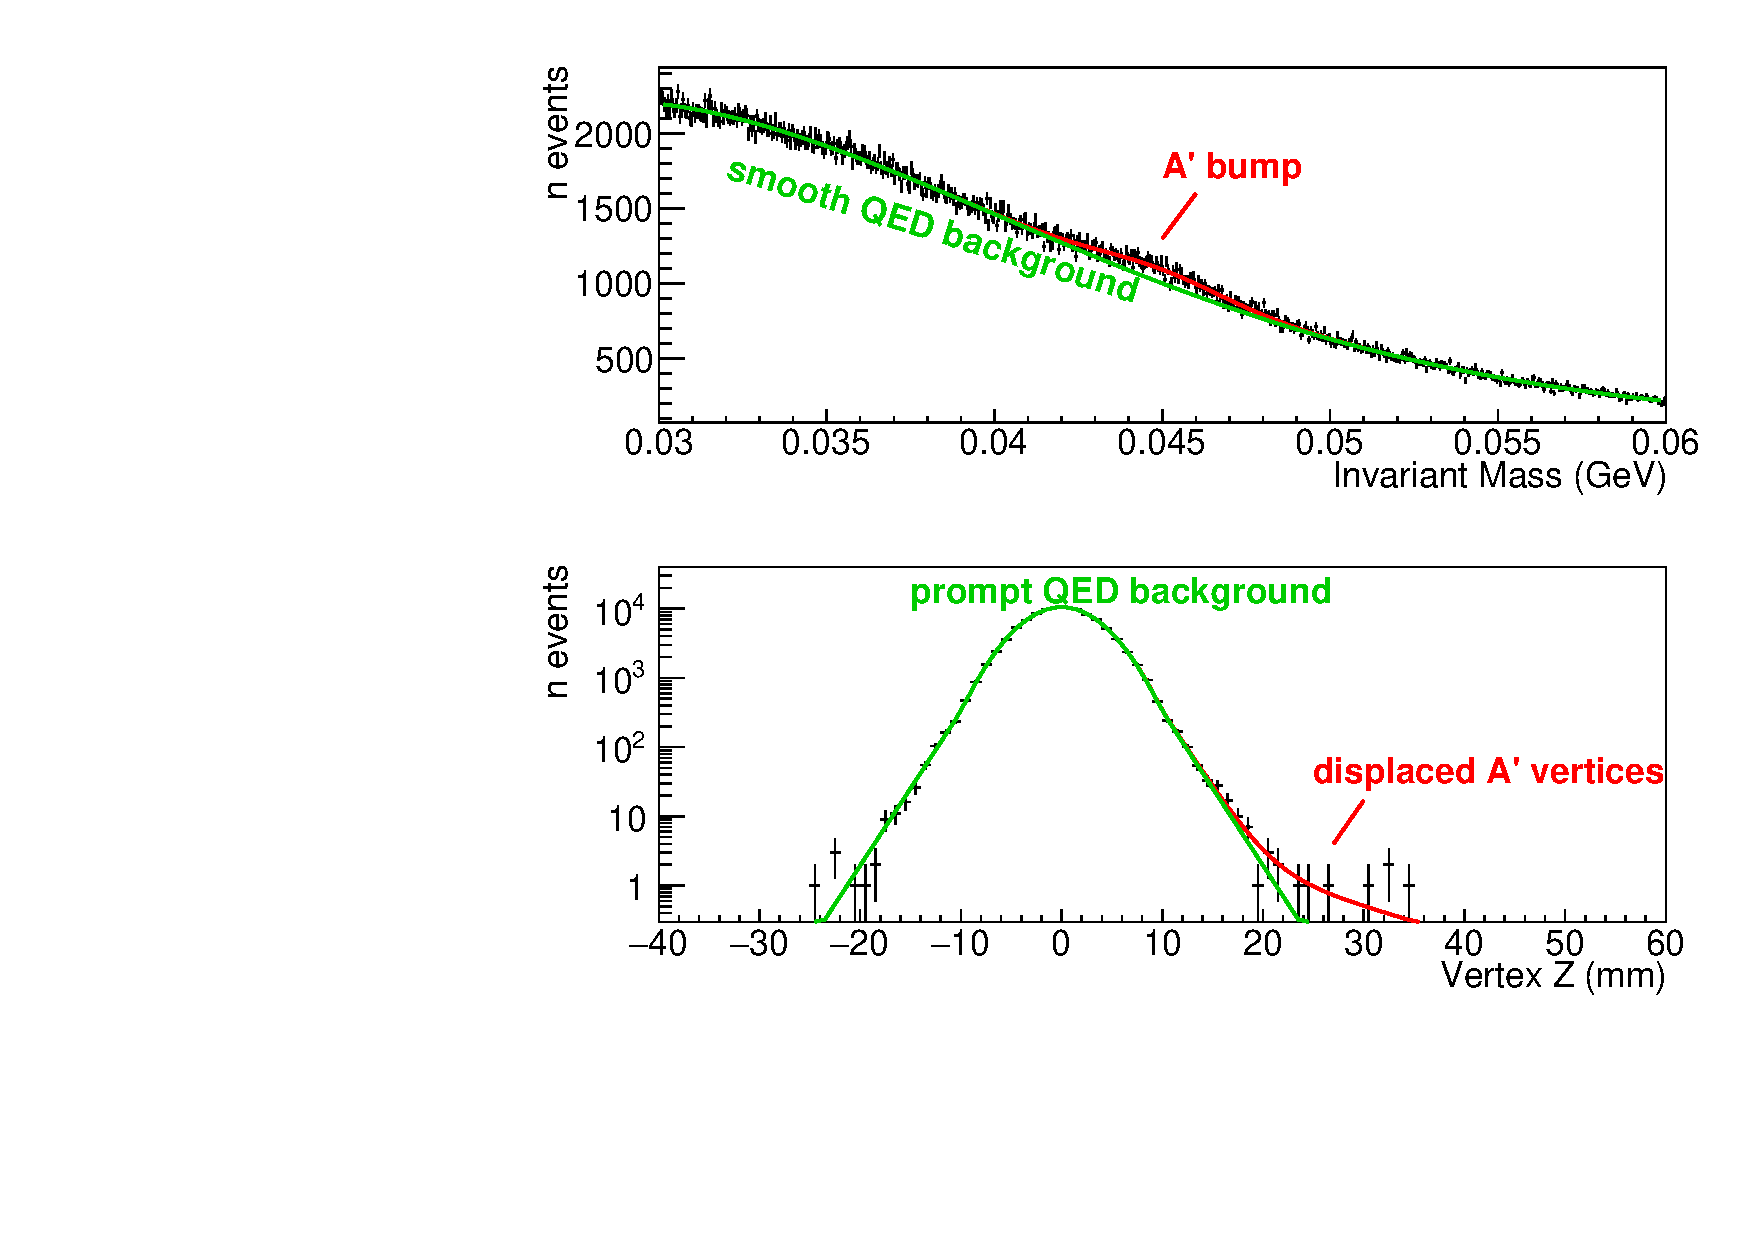
\includegraphics[width=1.1\textwidth,trim ={0 0.5cm 0.5cm 0},clip]{sig_examples}}
		\end{center}
		\caption{Example signals and backgrounds for (top) a resonance search and (bottom) a displaced-vertex search, with $\approx$ 5$\sigma$ significance.}
	\end{figure}

%Existing constraints (shaded, below) on an $A'$ come from a variety of sources, including
%\begin{itemize}
%\item electron and muon anomalous magnetic moment measurements 
%\item beam dump experiments
%\item other resonance-search experiments
%\end{itemize}

	\begin{figure}
		\begin{center}
			%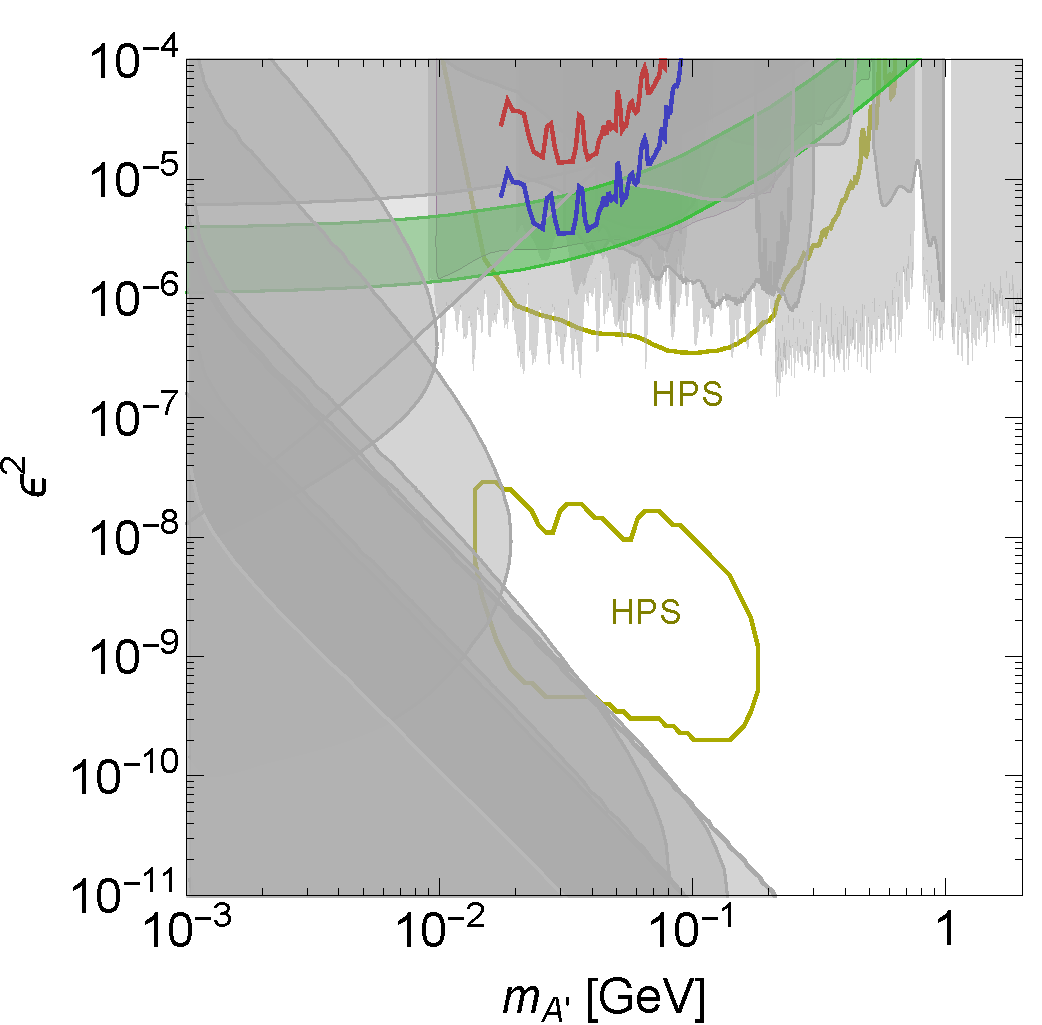
\includegraphics[width=0.9\textwidth]{reach_032017.pdf}
			%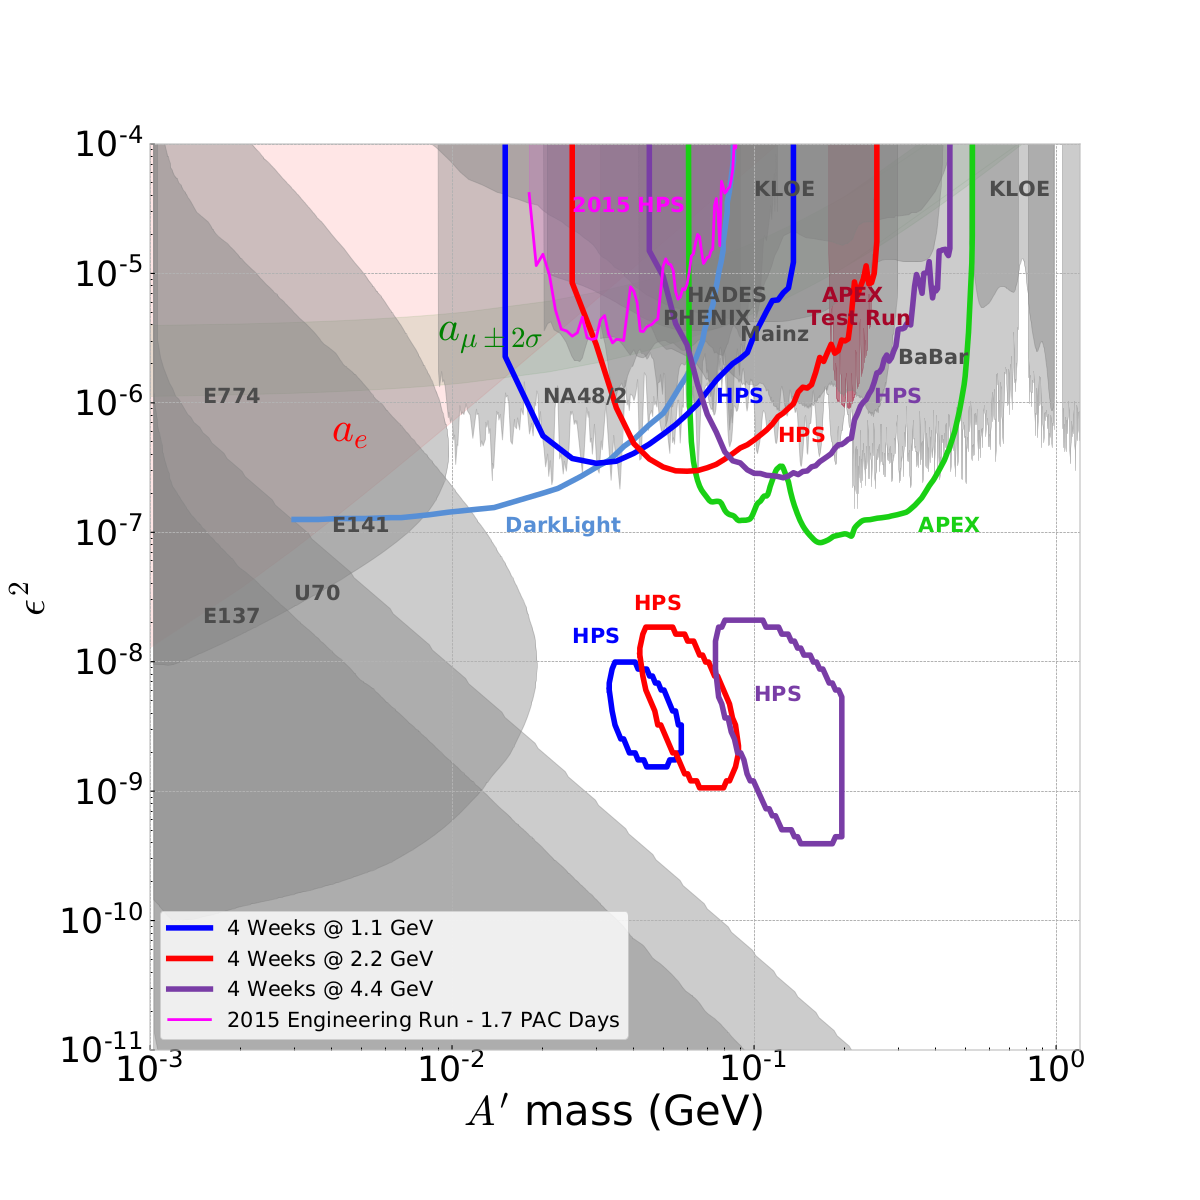
\includegraphics[width=1.0\textwidth]{reach_official_06_02_2017.png}

		
			%\makebox[\textwidth]
{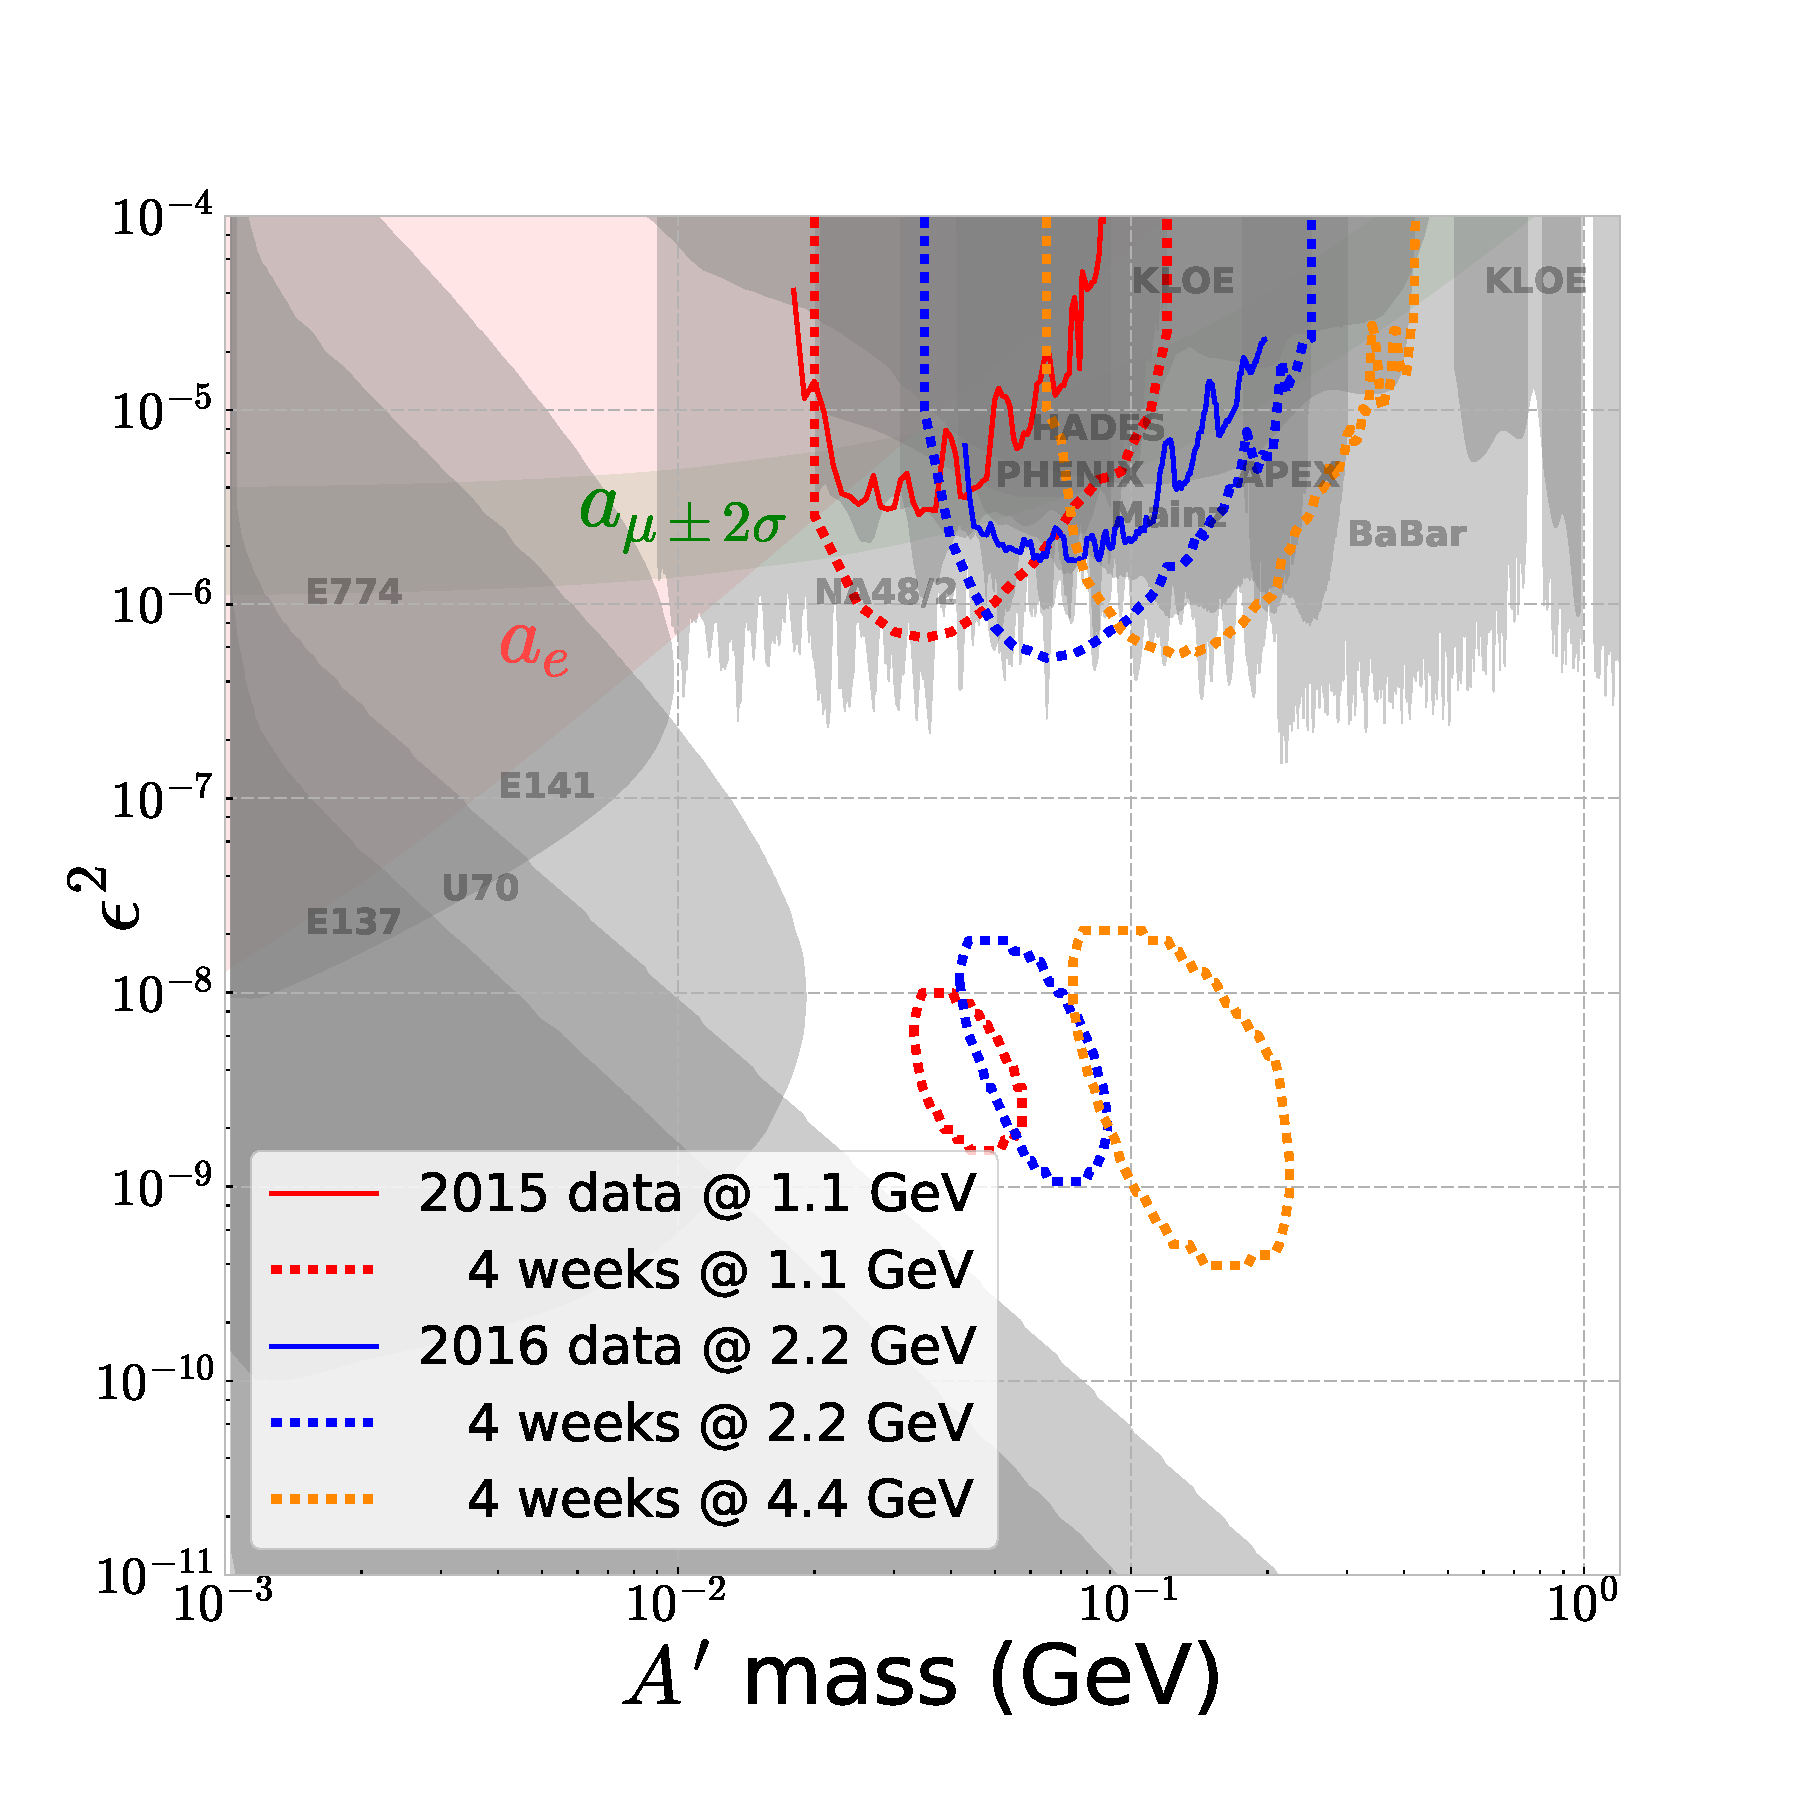
\includegraphics[trim={1.1cm 1cm -0cm 3cm},width=1.2\textwidth,clip]{reach/reach_new.pdf}}
		\end{center}
		\caption{Anticipated reach in $\alpha'/\alpha=\epsilon^2$ for HPS using existing data samples (solid lines) and larger future data samples (dashed).  
		 
}

	\end{figure}
	
	Existing constraints on the A' come from various other experiments, including beam-dumps, other resonance searches, and anomalous magnetic moments of electrons and muons. 
        \section*{Future of HPS}
%        \subsection*{Layer 0 Upgrade}
%        HPS is planning an upgrade to the SVT by adding another silicon tracking layer (Layer 0) between the target and 
%        first layer. This is expected to significantly improve the tracking of HPS in two main ways. First, it will improve the vertex resolution and hence 
%        the upward reach in the vertex search of HPS (lower solid brown lines in Fig. 9). Second, the upgrade will improve the detection 
%        efficiency of the recoil electron that will result in higher invariant mass resolution. This improves the overall experiment 
%        and especially the bump hunt reach.
%
%	\begin{figure}
%		\begin{center}
%			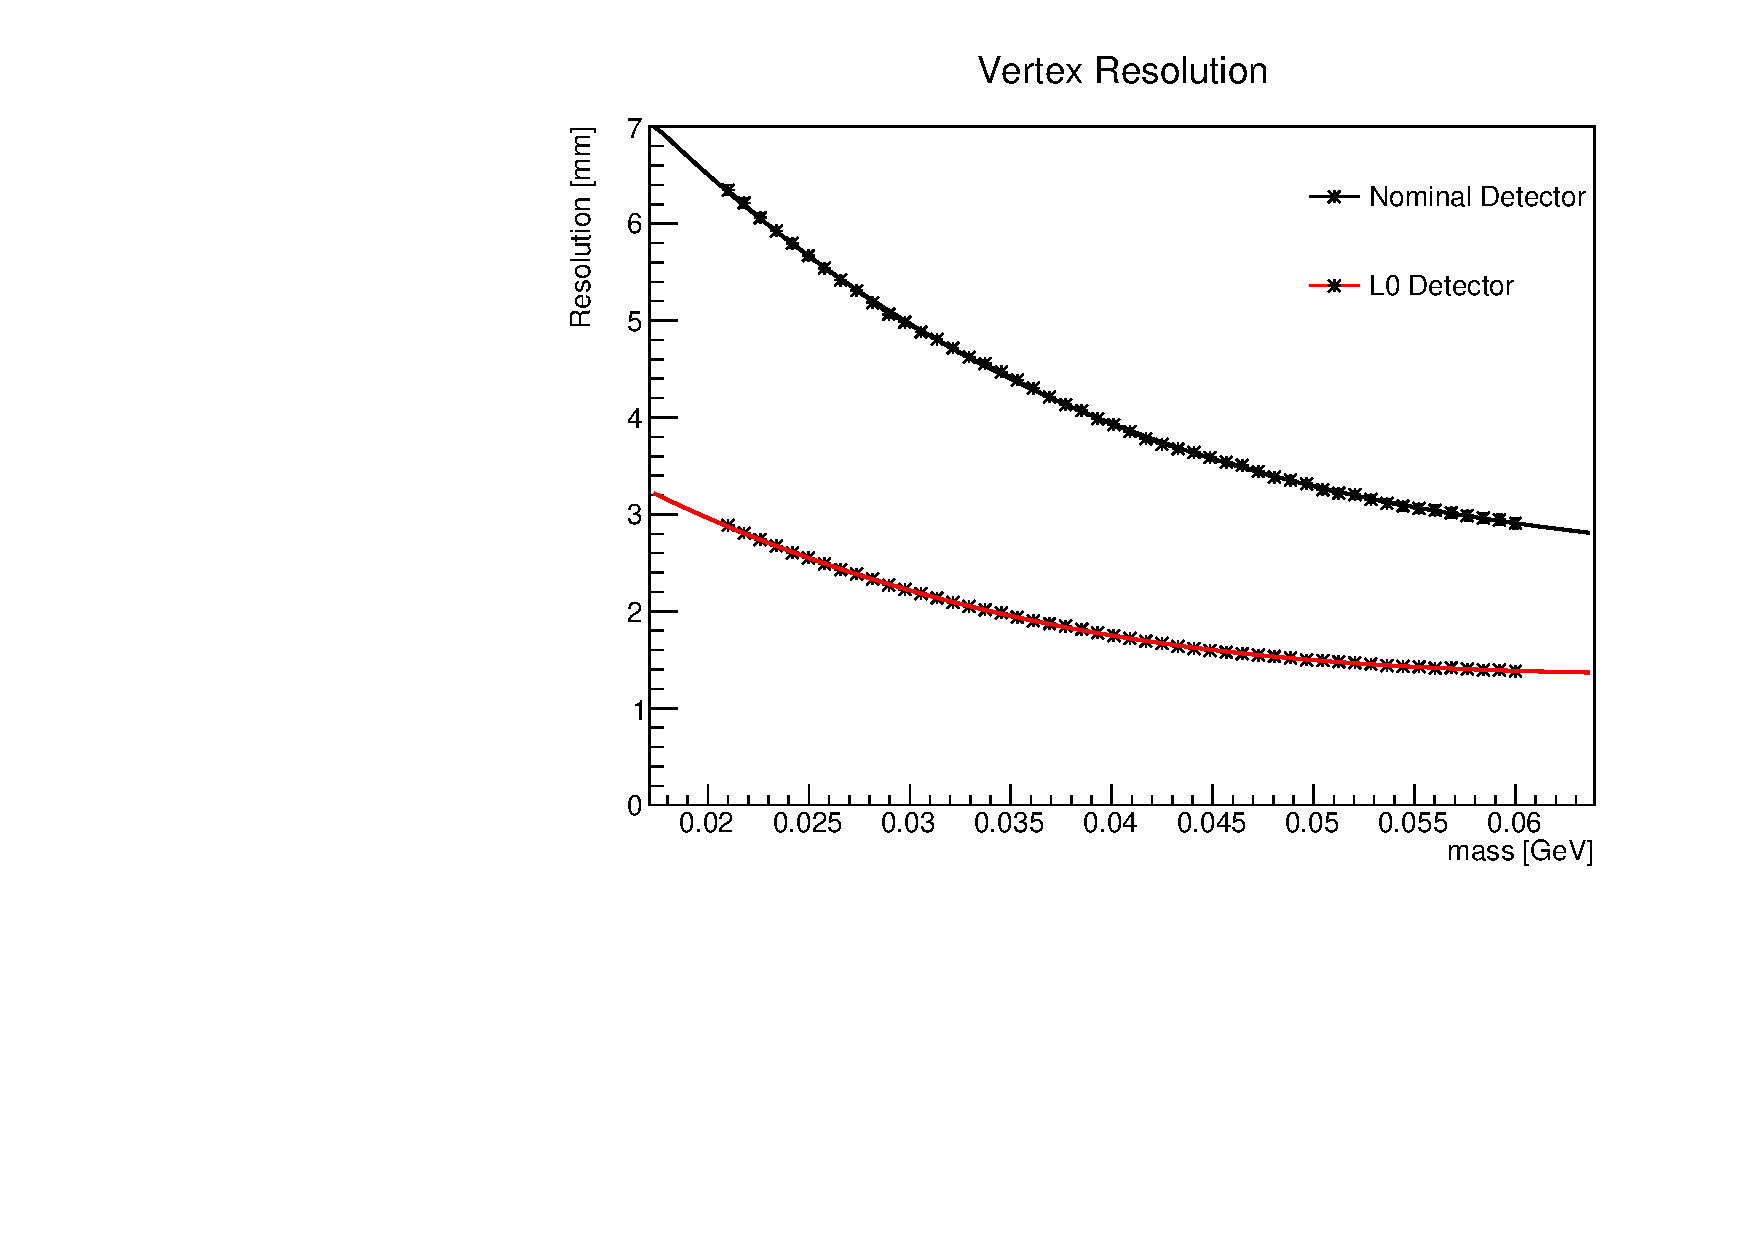
\includegraphics[width=0.75\textwidth]{Resolution.pdf}
%		\end{center}
%		\caption{A comparison of the vertex resolution between the nominal detector and the L0 upgrade detector shows an improvement of about a factor of about 2.}
%	\end{figure}

        %\subsection*{2018 Data Taking}
        The major physics results of HPS will result from the 2019 running, %and will produce several theses. HPS is currently looking for 
%        students (both rotation and permanent) for upgrades, data taking, and data analysis.
        with several proposed upgrades to improve the reach of the experiment through improved resolution and acceptance:  
        \begin{small}
     	\begin{itemize}
	\item Add a tracking ``layer 0" to the SVT,  between the target and the existing layer 1.  
	\item Add a hodoscope for an additional positron-only trigger.  
	\end{itemize}
	\end{small}
\end{multicols}
\end{document}
